\chapter{Wichtiger Anhang 1}

\begin{figure}[htb]
\centering		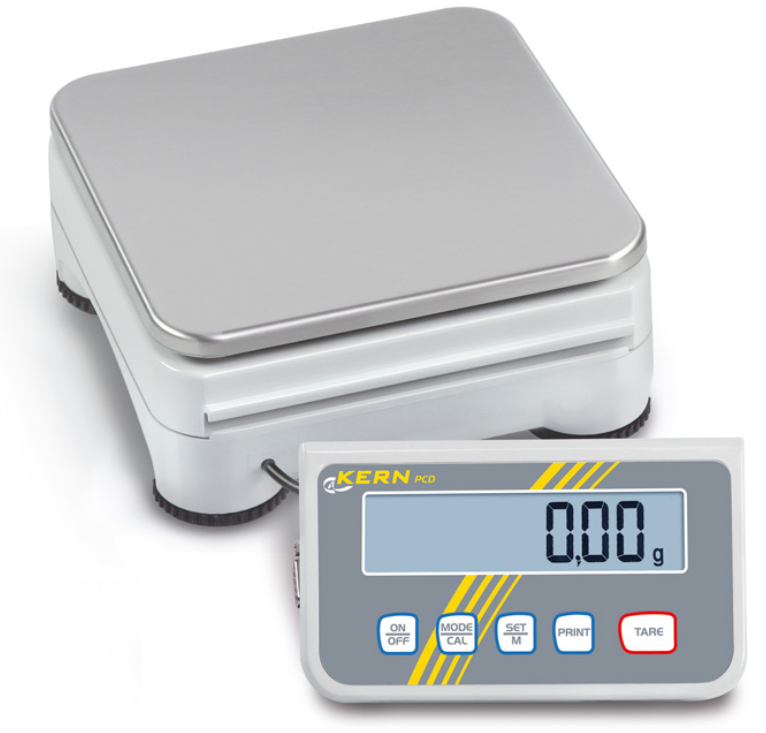
\includegraphics[width=0.50\textwidth]{Pictures/Waage.png}
\caption{Waage vom Typ \textit{PCD 10K0.1} der Fa. \textsc{Kern und Sohn Gmbh}}
\label{fig:}
\end{figure}

\begin{tabular}{cccccc}%{angle=90}
\hline 
\rule[-1ex]{0pt}{2.5ex} \textbf{Modbus Org.} & \textbf{EIA/TIA-485 Standard} & \textbf{Beckhoff/ TwinCat} & \textbf{Keller- Drucktransmitter} & \textbf{Krohne- Massenstromsensor} & \textbf{Carel-Expansionsventile} \\ 
\hline 
\rule[-1ex]{0pt}{2.5ex} D0 & Data A = Data (-) = inverted & Data (-) & RS 485 B & Signal A (D0) & (-) \\ 
\hline 
\rule[-1ex]{0pt}{2.5ex} D1 & Data B = Data (+) = non-inverted & Data (+) & RS 485 A & Signal B (D1) & (+) \\ 
\hline 
\rule[-1ex]{0pt}{2.5ex} Common & Common & Ground & GND & Common & GND \\ 
\hline 
\end{tabular} 
 

\section{Die Versalien}


\chapter{Ähnlich wichtiger Anhang}
